% ----------------------------------------------------------------- %
%             The Speech Signal Processing Toolkit (SPTK)           %
%             developed by SPTK Working Group                       %
%             http://sp-tk.sourceforge.net/                         %
% ----------------------------------------------------------------- %
%                                                                   %
%  Copyright (c) 1984-2007  Tokyo Institute of Technology           %
%                           Interdisciplinary Graduate School of    %
%                           Science and Engineering                 %
%                                                                   %
%                1996-2017  Nagoya Institute of Technology          %
%                           Department of Computer Science          %
%                                                                   %
% All rights reserved.                                              %
%                                                                   %
% Redistribution and use in source and binary forms, with or        %
% without modification, are permitted provided that the following   %
% conditions are met:                                               %
%                                                                   %
% - Redistributions of source code must retain the above copyright  %
%   notice, this list of conditions and the following disclaimer.   %
% - Redistributions in binary form must reproduce the above         %
%   copyright notice, this list of conditions and the following     %
%   disclaimer in the documentation and/or other materials provided %
%   with the distribution.                                          %
% - Neither the name of the SPTK working group nor the names of its %
%   contributors may be used to endorse or promote products derived %
%   from this software without specific prior written permission.   %
%                                                                   %
% THIS SOFTWARE IS PROVIDED BY THE COPYRIGHT HOLDERS AND            %
% CONTRIBUTORS "AS IS" AND ANY EXPRESS OR IMPLIED WARRANTIES,       %
% INCLUDING, BUT NOT LIMITED TO, THE IMPLIED WARRANTIES OF          %
% MERCHANTABILITY AND FITNESS FOR A PARTICULAR PURPOSE ARE          %
% DISCLAIMED. IN NO EVENT SHALL THE COPYRIGHT OWNER OR CONTRIBUTORS %
% BE LIABLE FOR ANY DIRECT, INDIRECT, INCIDENTAL, SPECIAL,          %
% EXEMPLARY, OR CONSEQUENTIAL DAMAGES (INCLUDING, BUT NOT LIMITED   %
% TO, PROCUREMENT OF SUBSTITUTE GOODS OR SERVICES; LOSS OF USE,     %
% DATA, OR PROFITS; OR BUSINESS INTERRUPTION) HOWEVER CAUSED AND ON %
% ANY THEORY OF LIABILITY, WHETHER IN CONTRACT, STRICT LIABILITY,   %
% OR TORT (INCLUDING NEGLIGENCE OR OTHERWISE) ARISING IN ANY WAY    %
% OUT OF THE USE OF THIS SOFTWARE, EVEN IF ADVISED OF THE           %
% POSSIBILITY OF SUCH DAMAGE.                                       %
% ----------------------------------------------------------------- %
\hypertarget{lsp2sp}{}
\name{lsp2sp}{transform LSP to spectrum}
{speech parameter transformation}

\begin{synopsis}
\item[lsp2sp] [ --m $M$ ] [ --s $S$ ] [ --l $L$ ] [ --L ] [ --k ] [ --q $Q$ ] [ --o $O$ ] [ {\em infile} ]
\end{synopsis}

\begin{qsection}{DESCRIPTION}
{\em lsp2sp} calculates the spectrum from the line spectral pairs (LSP)
from {\em infile} (or standard input),
sending the result to standard output.

Input and output data are in float format.

The LSP input format is
 \begin{displaymath}
  [ K ], l(1), \dots, l(M).
 \end{displaymath}
The spectrum can be obtained by
  \begin{displaymath}
   \mid H(\mathrm{e}^{-j\omega}) \mid = \frac{K}{\mid A_p(\mathrm{e}^{-j\omega}) \mid}.
  \end{displaymath}
where $\mid A_p(\mathrm{e}^{-j\omega}) \mid$ is given as follows:

When the order of LSP is even, 
  \begin{displaymath}
   \mid A_p(\mathrm{e}^{-j\omega}) \mid = \sqrt{ 2^M \left\{ \cos^2 \frac{\omega}{2}\prod_{i=1,3,\cdots,M-1}(\cos \omega - \cos l(i))^2 + \sin^2 \frac{\omega}{2}\prod_{i=2,4,\cdots,M}(\cos \omega - \cos l(i))^2 \right\} }.
  \end{displaymath}
When the order of LSP is odd,
 \begin{displaymath}
  \mid A_p(\mathrm{e}^{-j\omega}) \mid = \sqrt{ 2^{M-1} \left\{ \prod_{i=1,3,\cdots,M}(\cos \omega - \cos l(i))^2 + \sin^2 \omega \prod_{i=2,4,\cdots,M-1}(\cos \omega - \cos l(i))^2 \right\} }.
 \end{displaymath}
\end{qsection}

\begin{options}
 \argm{m}{M}{order of LSP}{10}
 \argm{s}{S}{sampling frequency (kHz)}{10.0}
	\argm{l}{L}{frame length}{256}
 \argm{L}{}{regard input log gain as linear one}{FALSE}
 \argm{k}{}{input gain}{TRUE}
	\argm{q}{Q}{input format\\
        \begin{tabular}{ll} \\[-1ex]
            $0$ & normalized frequency $(0 \dots \pi)$ \\
            $1$ & normalized frequency $(0 \dots 0.5)$ \\
            $2$ & frequency (kHz) \\
            $3$ & frequency (Hz)  \\
        \end{tabular}\\\hspace*{\fill}}{0}
	\argm{o}{O}{output format\\
 \begin{tabular}{ll} \\[-1ex]
  $0$ & $20 \times \log |H(z)|$ \\
  $1$ & $\ln |H(z)|$ \\
  $2$ & $|H(z)|$ \\
  $3$ & $|H(z)|^{2}$ \\[1ex]
 \end{tabular}\\\hspace*{\fill}}{0}
\end{options}

\begin{qsection}{EXAMPLE}
The example below takes the 15-th order LSP from the file
 {\em data.lsp} in float format, evaluates the spectrum,
 and presents it in the screen:
\begin{quote}
 \verb! lsp2sp -m 15 data.lsp | glogsp -x 5 | xgr ! 
\end{quote}
\begin{center}
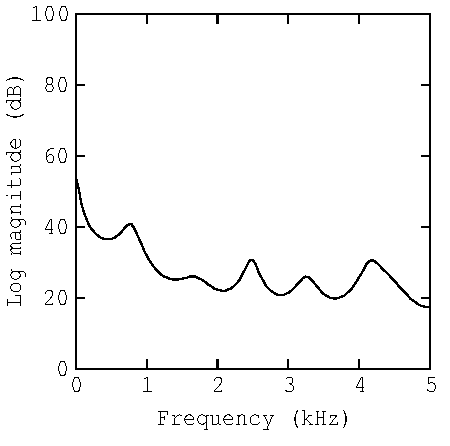
\includegraphics[width=6cm]{fig/lsp2sp.pdf}
\end{center}
\end{qsection}

\begin{qsection}{SEE ALSO}
\hyperlink{lpc2lsp}{lpc2lsp},
\hyperlink{lspcheck}{lspcheck}
\end{qsection}
